%%%%%%%%%%%%%%%%%%%%%%%%%%%%%%%%%%%%%%%%%%%%%%%%%%%%%%%%%%%%%%%%%%%%%%%%%%%%%%%%%%%%%%%%%%%%
%%
%% Chapter 4 : Proposal
%%
%%      * Should give a more detailed explanation of the proposal
%%
%%  BASIC STRUCTURE :
%%
%%      a. Framework overview
%%          * Why yet another framework ?
%%          * Architecture
%%
%%      b. Framework Components
%%          * Core
%%              > Agents API
%%              > Terrain API
%%              > Sensors API
%%              > Tasks API
%%          * Backends
%%          * User API via Python bindings
%%          * Extensions
%%
%%      c. Baseline implementations
%%
%%
%%%%%%%%%%%%%%%%%%%%%%%%%%%%%%%%%%%%%%%%%%%%%%%%%%%%%%%%%%%%%%%%%%%%%%%%%%%%%%%%%%%%%%%%%%%%

\chapter{Detailed description of the Proposal}
\label{ch:proposal}

%%%%%%%%%%%%%%%%%%%%%%%%%%%%%%%
%   Figures for chapter 4
%%%%%%%%%%%%%%%%%%%%%%%%%%%%%%%

\newcommand{\figProposalComparison}{
    \begin{figure}
        \centering
        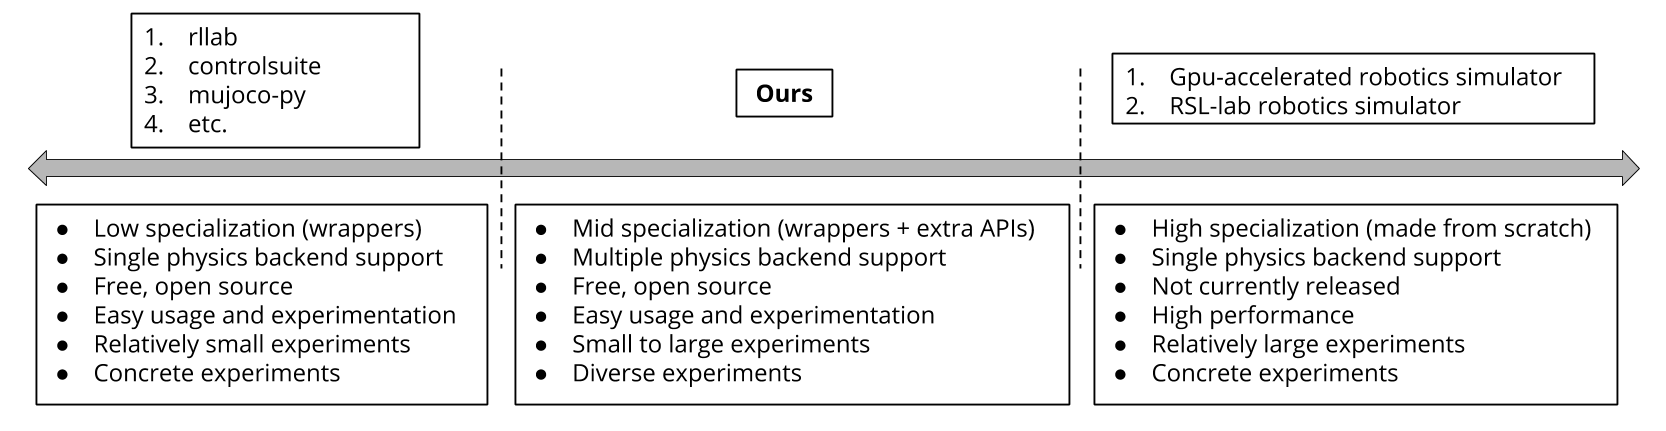
\includegraphics[width=1.0\textwidth]{./chapters/chapter_4/imgs/img_proposal_comparison.png}
        \caption{A comparison of our proposal with currently available benchmarks.}
        \label{fig:ch4_proposal_comparison}
    \end{figure}
}

As explained in chapter 1, where we presented the proposal, this thesis is mainly
focused in making a framework for evaluation of Deep Reinforcement Learning based agents
in diverse and complex environments. This chapter will give more details about the 
proposal for this thesis. We split the discussion in this chapter into the following two sections: 

\begin{itemize}
    \item Details of the proposed framework, where we discuss the core functionality 
          of the framework, the architecture to be used, and the extends of the framework.
    \item Details of the evaluation experiments, where we discuss the proposed experiments
          that will be implemented as part of this thesis.
\end{itemize}

\section{Details of the proposed framework}

The framework proposed consists basically of a multi-backend framework with some
APIs exposed to the user to handle tasks creation and setup. The framework is multi-backend
in the sense that it provides the user with the ability to choose to run their experiments
in a range of supported physics backends, like MuJoCo, Bullet, PhysX and FleX. We take
this approach to provide the user with more flexibility on the choice of the platform because
each backend has specific advantages and disadvantages. A description of the steps involved 
when creating a task with the proposed framework is shown in Figure @FIG-4.1, which consist of:

\begin{itemize}
    \item \textbf{User functionality} to describe the task. A description of the task is given by 
          the agents to be used, terrain generation configurations, sensors to be used, etc. This configuration
          can be passed by the user via a configuration file or programmatically.
    \item \textbf{Core functionality} used to create core data structures that will be used by the framework.
          The core data structures used involve the agents, terrain generators, sensors, and tasks. These are
          abstract in the sense that are not dependent of the specific backend (backend agnostic).
    \item \textbf{Backend-specific functionality} used to instantiate the required core representations
          into the specific resources needed for each backend. We model these are some set of \textbf{adapters}
          that can be \textbf{swapped} (dynamically loaded) depending of the choice of backend.
\end{itemize}

\figFrameworkFlow

In order to take into account the features proposed (multi-backend and diverse environment
creation) we decided to use the architecture shown in Figure @FIG-4.2. We separete the core
functionality into different modules, and create adapters for each backend (similar to wrappers) 
around the base structures in each core module. These adapters are in charge of instantiating the
necessary resources required by the base core structures. The framework then exposes the core
functionality (which is linked to the backend specific functionality) to the user via the tasks
that were created. The user can then interact with all aspects of the simulation, e.g. setting
control commands, via these created tasks.

Notice that there is a similar group of adapters that are used by the rendering backend. We
decided to take the same multi-backend approach for the visualizer because there are various situations
in which we could potentially need to choose between different rendering backends, like using a 
headless rendering backend in servers with no windowing system initialized, or using a photorealistic
rendering backend to make different experiments when trying to do more complicated simulations related to
the real world.

\figFrameworkArchitecture

\subsection{Core functionality}

The core functionality consists of the core data structures used to represent agents,
terrain and sensors, which are decoupled from the specific backends to be used. This functionality
is composed of the following components:

\begin{itemize}
    \item \textbf{Agents representations}: these representations consist of the core kinematric tree and its
          variants. These variants could in principle model different situations that could be needed
          for some specific task. All these representations are abstract, and their components (bodies, 
          joints, collisions, etc.) are decoupled from the specific resources provided in the backends.
          These representations are also decoupled from the specific format used to store the kinematic
          tree in disk. The formats we are considering include \textit{urdf}, \textit{mjcf}, and custom
          formats through .xml and .json files. All this functionality is summarized in Figure @FIG-4.3.

    \item \textbf{Terrain representations}: these representations consist of the core terrain generator and its
          variants. These variants model the different types of terrain that one could need. In principle
          there are a few core generators, which are in charge of creating various environments. These core
          generators consist of procedural and static generators. Procedural generators are used for creating
          different terrain during runtime, and static generators are used to create a static scene and task
          with no changes in the terrain. The terrain generators will create abstract "primitives" which can then
          be used to create the desired terrain resources using the selected backend. These primitives are the minimal
          terrain resource that can be used, and consist of geometric primitives, mesh objects representing heightmaps,
          and other minimal objects that could be needed for more specific tasks. All this functionality is
          summarized in Figure @FIG-4.4.

    \item \textbf{Sensors representations}: these representations consist of the core sensors that will be exposed
          to the user in order to train an agent. This are also abstract, and get the information from the
          core agents and terrain generators. The type of sensors that will be implemented are: joint readings (angles 
          and speeds), body readings (relative position to root body, linear velocities and accelerations), 
          heightmap readings of the terrain, and camera readings in the form of RGB frames. The proposed sensors are shown
          in Figure @FIG-4.5.
\end{itemize}

\subsection{Specific implementations for different backends}

%% @TODO: Talk about approach of using adapters

The backend-specific functionality is in charge of instantiating the appropiate 
resources in the given backend, like instantiating bodies and joints for the abstract 
agents, creating the appropiate terrain resources from the terrain primitives, and storing
the required sensor readings that will be grabbed afterwards by each abstract sensor.

The approach we chose is to use adapters for the core functionality. These adapters
will link the specific backend functionality to the abstract resource. This is why
extra care has to be placed in flexible abstract representations because each backend
should be able to support this functionality. Then, it is only necessary to write
the adapters for the base abstract representations.

For example, if we had various terrain generators for specific variations that one
might need in a specific task, all these terrain generators end up creating primitives.
These primitives are the blueprints that the adapter can then use to instantiate that given
terrain in the specific backend. A similar approach is used for the rest of the core
functionality, where the adapters use the component blueprints provided by the core data structures.
This mix of composition and adaptation is often called the \textit{Bridge pattern}, and it is
often used when decoupling platform specific functionality from core functionality, e.g. when
abstracting libraries for different operating systems. The user is then only exposed to
the abstract functionality which should act as a bridge to the specific backend, as shown in
Figure @FIG-4.6.

%% \figBridgePattern

%% @TODO: Talk about how will everything work (dlinking)

Another detail to take into account is how to support multiple and swappable backends
for the user. To achieve this we will make use of runtime library loading. This allows us
to load the specific backend library at runtime as specified by the user, and it is an OS specific
feature usually provided in the context of dynamic linking. To fully integrate
this feature into the framework the only change that has to be made is to expose the user 
to \textit{base adapters}, which can then be loaded with the specific adapters using runtime loading.
This process is shown in Figure @FIG-4.7.

%% \figRuntimeLibraryLoading


%% @TODO: Explain about the proposed supported backends (mujoco, bullet, physx, flex)

The choice of supporting multiple backends was made because of the advantages and
disadvantages that each physics backend has. For example, PhysX 4.0 has features that
allow it to run large number of simulated agents, FleX can be used when trying to
create fluid manipulation tasks, MuJoCo can be used for more precise simulations, and
Bullet can be used for the same tasks provided by MuJoCo, but without the need to have
a license for extended usage.

\subsection{Construction APIs}

@TODO: Talk about the terrain APIs that will be provided to create terrain

@TODO: Talk about the tasks APIs that will be provided to create tasks

@TODO: Talk about the user APIs that will be provided in python to the user for
       even easier usage and experimentation

\section{Details of the proposed evaluations and baselines}

@TODO: Talk about the algorithms to be used from the current state of the art.

\subsection{Base experiments}

@TODO: Talk about the vanilla experiments to be implemented, which should
       consist of the learning environments without a given curricula (just use
       the new environments and see how well an state-of-the-art agent does)

\subsection{Imitation experiments}

@TODO: Talk about the experiments to be implenented that take into account some
       form of imitation. This should include agents that can be learned using 
       available mocap data and keyframe authored animations.

\subsection{Hard-coded curricula experiments}

@TODO: Talk about the experiments to be implemented that make use of some form
       of curricula, e.g using simple procedural generation via random ranges.

\subsection{Adaptive curricula experiments}

@TODO: These experiments are some ideas that I want to ponder and see how to implement
       in the future. As I stated in the hypothesis, we should try some form of
       adaptive curricula that based on the performance of the agent it would create
       the terrain and task appropiately in order to encourage better learning. This
       would be some kind of "training-wheels" module that could be hard-coded or even 
       learned from experience. In my mind it sounds like and actor-supervisor approach,
       in which the supervisor sets the terrain generator paraeters using the provided API
       according to how well the agent is doing. This could be done in stages, switching between
       a hard-coded curricula and the adaptive curricula.

